% Generated by scripts/make_census_figures.py -- do not edit by hand.
\begin{tikzpicture}[x=1cm, y=1cm,
  axis/.style={draw=black!75, line width=0.4pt},
  nonsum/.style={draw=black, line width=0.9pt},
  sum/.style={draw=black!45, line width=0.6pt},
  lead/.style={draw=black!35, line width=0.3pt},
]
  \fill[black!8] (0,0) rectangle (6.979,2.70);
  \draw[axis, densely dashed] (6.979,0) -- (6.979,2.70);
  \node[font=\scriptsize, anchor=south east, black!55] at (6.879,2.42) {conjectured gap: no class here};
  \draw[axis] (0,0) -- (12.00,0);
  \node[font=\scriptsize, anchor=north] at (0,-0.08) {$\tfrac13$};
  \node[font=\scriptsize, anchor=north] at (12.00,-0.08) {$\tfrac9{25}$};
  \draw[sum] (7.075,0) -- (7.075,0.576);
  \draw[lead] (7.075,0.576) -- (7.045,1.02);
  \node[font=\tiny, anchor=west, inner sep=1pt, fill=white, fill opacity=.9, text opacity=1] at (7.075,1.02) {$\frac{37}{106}$\,{\scriptsize$\times$}11};
  \draw[sum] (7.581,0) -- (7.581,0.401);
  \draw[lead] (7.581,0.401) -- (7.045,1.62);
  \node[font=\tiny, anchor=west, inner sep=1pt, fill=white, fill opacity=.9, text opacity=1] at (7.075,1.62) {$\frac{97}{277}$\,{\scriptsize$\times$}3};
  \draw[nonsum] (7.655,0) -- (7.655,0.290);
  \draw[lead] (7.655,0.290) -- (7.045,2.22);
  \node[font=\tiny, anchor=west, inner sep=1pt, fill=white, fill opacity=.9, text opacity=1] at (7.075,2.22) {$\frac{254}{725}$$^{\ast}$\,{\scriptsize$\times$}1};
  \draw[sum] (7.701,0) -- (7.701,0.355);
  \draw[lead] (7.701,0.355) -- (9.295,1.02);
  \node[font=\tiny, anchor=west, inner sep=1pt, fill=white, fill opacity=.9, text opacity=1] at (9.325,1.02) {$\frac{157}{448}$\,{\scriptsize$\times$}2};
  \draw[sum] (7.895,0) -- (7.895,0.490);
  \draw[lead] (7.895,0.490) -- (9.295,1.62);
  \node[font=\tiny, anchor=west, inner sep=1pt, fill=white, fill opacity=.9, text opacity=1] at (9.325,1.62) {$\frac{20}{57}$\,{\scriptsize$\times$}6};
  \draw[nonsum] (8.733,0) -- (8.733,0.355);
  \draw[lead] (8.733,0.355) -- (9.295,2.22);
  \node[font=\tiny, anchor=west, inner sep=1pt, fill=white, fill opacity=.9, text opacity=1] at (9.325,2.22) {$\frac{103}{292}$$^{\ast}$\,{\scriptsize$\times$}2};
  \draw[nonsum] (8.745,0) -- (8.745,0.355);
  \draw[sum] (8.824,0) -- (8.824,0.722);
  \draw[sum] (8.922,0) -- (8.922,0.355);
  \draw[sum] (9.231,0) -- (9.231,0.649);
  \draw[sum] (9.437,0) -- (9.437,0.401);
  \draw[nonsum] (9.623,0) -- (9.623,0.355);
  \draw[sum] (9.736,0) -- (9.736,0.436);
  \draw[sum] (10.000,0) -- (10.000,0.727);
  \draw[sum] (10.130,0) -- (10.130,0.490);
  \draw[sum] (10.274,0) -- (10.274,0.576);
  \draw[sum] (10.443,0) -- (10.443,0.401);
  \draw[nonsum] (10.526,0) -- (10.526,0.290);
  \draw[sum] (10.714,0) -- (10.714,0.900);
  \draw[sum] (10.766,0) -- (10.766,0.436);
  \draw[nonsum] (10.794,0) -- (10.794,0.290);
  \draw[sum] (10.800,0) -- (10.800,0.490);
  \draw[sum] (10.830,0) -- (10.830,0.490);
  \draw[sum] (10.837,0) -- (10.837,0.490);
  \draw[nonsum] (11.057,0) -- (11.057,0.355);
  \draw[sum] (11.111,0) -- (11.111,0.649);
  \draw[sum] (11.290,0) -- (11.290,0.490);
  \draw[nonsum] (11.381,0) -- (11.381,0.355);
  \draw[nonsum] (11.435,0) -- (11.435,0.290);
  \draw[nonsum] (11.437,0) -- (11.437,0.290);
  \draw[sum] (11.538,0) -- (11.538,0.827);
  \draw[sum] (11.569,0) -- (11.569,0.490);
  \draw[sum] (11.638,0) -- (11.638,0.436);
  \draw[nonsum] (11.693,0) -- (11.693,0.290);
  \draw[nonsum] (11.722,0) -- (11.722,0.290);
  \draw[sum] (11.818,0) -- (11.818,0.490);
  \draw[sum] (11.826,0) -- (11.826,0.355);
  \draw[sum] (11.842,0) -- (11.842,0.490);
  \draw[sum] (11.871,0) -- (11.871,0.727);
  \draw[sum] (11.921,0) -- (11.921,0.355);
  \draw[sum] (11.960,0) -- (11.960,0.436);
  \draw[sum] (12.000,0) -- (12.000,0.859);
\end{tikzpicture}
% caption: 42 distinct balance constants of order-14 posets lie in $(1/3, 9/25]$.  Stem height grows with the number of classes attaining the value.  36 further values are drawn but not labelled.  
